\chapter{Neural Networks}
The goal of this appendix is to give a simple albeit incomplete introduction of
Neural Networks for those readers who have not a solid background on it but
still they are interested in Chapter \ref{wordemb}.

\section{Gradient descent}
Given a minimization problem $min_w f(w), w \in \mathbb{R}^D$,
it is possible to find a local minimum through gradient descent.

First, we compute the gradient $\nabla f(w)$ and we decide a point $w_0$ in which the algorithm has to start.
If the problem is not convex, choosing a different $x_0$ could lead to a different
solution.
Since gradients point in the direction of fastest increase,
we take small steps towards the opposite direction in order to reach a minimum.

The step size is controlled by a hyperparameter $\lambda$:
values too small for a particular problem increase
the time needed to obtain a good solution and
it can lead to a local minimum;
values too big prevent convergence.

The final equation is:
$$ w_{i+1} = w_{i} - \lambda \nabla f(w_i) $$

Each step is run iteratively until a stopping criterion is met.
If the algorithm is stopped after $I$ iterations, the solution
for the minimization problem is $w_{I}$.
Common sense stopping criterions could be:
\begin{itemize}
    \item stop after a prefixed number of iterations
    \item stop when the results are not getting better for the last $I$ steps
    \item stop when $f(w_i) - f(w_{i+1}) < \epsilon$, with $\epsilon > 0$ small
\end{itemize}

Note that the parameter $\lambda$ could be different at each iteration:
$$ w_{i+1} = w_{i} - \lambda_{i+1} \nabla f(w_i) $$
For instance, we could have $\lambda_i = \frac{\lambda}{i}$ in order to take
smaller and smaller steps until convergence.

\subsection{Gradient descent in action} \label{gradesc}
Suppose to have a dataset $X \in \mathbb{R}^{N \times D}, y \in \mathbb{R}^N$.

What we want to do is linear regression, whose model is obtained resolving:
$$\displaystyle \min_{w \in \mathbb{R}^D} \frac{1}{2N} \sum_{i \in [1, N]} (w^T x_i - y_i)^2$$

The derivative  $\frac{1}{2N} \sum_i (w^T x_i - y_i)^2 dw$ is:
$$\frac{1}{2N} \sum_{i \in [1, N]} 2 x_i(w^T x_i - y_i) = \frac{\sum_{i \in [1, N]} x_i(w^T x_i - y_i)}{N}$$

Therefore:
$$ w_{n+1} = w_n - \frac{\lambda}{N} \sum_{i \in [1, N]} x_i(w_i^T x_i - y_i) $$


\section{Mini-batch gradient descent}
There are situations in which using gradient descent is not computationally feasible.
For instance, imagine that the problem explained in Section \ref{gradesc} have
a number of points so huge that a solution can not be obtained in feasible times.

Mini-batch gradient descent is an extension of gradient descent which assume that
samples of $|M|$ elements of the dataset are a noisy representative of the entire data.
At each step, $M$ will be re-sampled from $X$.

In that case, the minimization presented in Section \ref{gradesc} can be rewritten as:
$$\displaystyle \min_{w \in \mathbb{R}^D} \frac{1}{2|M|} \sum_{x_i \in M} (w^T x_i - y_i)^2 $$

\section{Linear Neural Networks}
The linear regression exposed in Section \ref{gradesc} can be viewed as a Neural Network
which has $D$ inputs as a first layer and a single neuron as output connected to all previous ones.

The graphical representation of it can be seen in Figure \ref{fig:nn-linear}.

The vector $w$ is simply the set of all weights.
Starting from the equation presented in Section \ref{gradesc}:
$$ w_{n+1} = w_n - \frac{\lambda}{N} \sum_{i \in [1, N]} x_i(w^T x_i - y_i) $$
each weight $w_i$ can be parallelly updated:
$$ w_{(n+1)j} = w_{nj} -  \frac{\lambda}{N} \sum_{i \in [1, N]} x_{ij}(w^T x_i - y_i) $$

In this example, the cost function is the square loss, but there is not any particular requirement when
dealing with Neural Networks.

\begin{figure}[h]
    \centering
    \subfigure{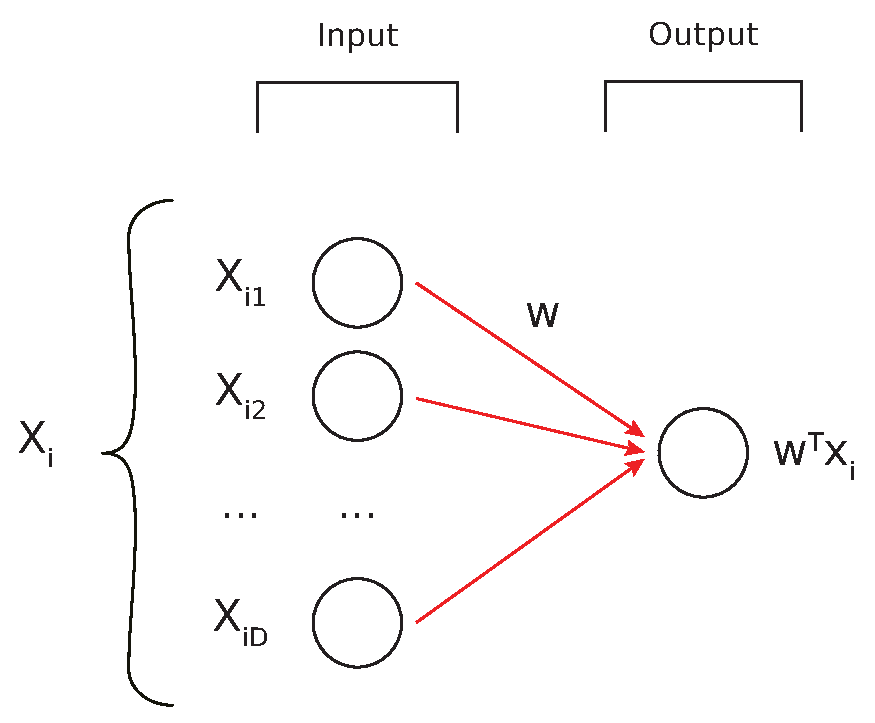
\includegraphics[width=0.5\textwidth]{images/nn-linear.eps}}
    \caption{A graphical representation of a linear Neural Network.}
    \label{fig:nn-linear}
\end{figure}

\section{Activation functions}
In each node, a non-linear function could be applied at the data before moving the output to the next layer.
For the sake of simplicity, we are going to present a model similar to the previous one,
with the difference that a $\tanh(\cdot)$ function is applied to the output node:
$$ \displaystyle \min_{w \in \mathbb{R}^D} \frac{1}{2N} \sum_{i \in [1, N]} [\tanh(w^T x_i) - y_i]^2 $$

To resolve it with gradient descent, we have to apply the chain rule.
Since $\tanh(z) dz = 1 - tanh^2(z)$:
$$ \frac{1}{2N} \sum_{i \in [1, N]} [\tanh(w^T x_i) - y_i]^2 dw =
    \frac{1}{2N} \cdot \sum_{i \in [1, N]} 2[\tanh(w^T x_i) - y_i] \cdot [1 - tanh^2(w^T x_i)] \cdot x_i $$
$$ w_{n+1} = w_n -
    \frac{\lambda}{N} \sum_{i \in [1, N]} [\tanh(w^T x_i) - y_i] [1 - tanh^2(w^T x_i)] x_i $$

Other activation functions can be used instead of $\tanh(\cdot)$.
The one used in the models presented in Chapter \ref{wordemb} is the softmax
$\sigma(z), z \in \mathbb{R}^V$:
$$\sigma(z, j) =  \frac{e^{z_i}}{\sum_j e^{z_j}}$$
$$ \sigma(z) =
    \begin{bmatrix}
        \sigma(z, 1) \\ \sigma(z, 2) \\ ... \\ \sigma(z, V)
    \end{bmatrix}
$$

\section{Multilayer Neural Networks}
Adding intermediate layers (usually called hidden layers in the literature)
to a linear Neural Network is useless
since the product of linear components is again linear.
As an example, construct a model with the following characteristics:
\begin{itemize}
    \item $X \in \mathbb{R}^{N \times 2}$: 2 nodes as input
    \item $y \in \mathbb{R}^N$: 1 node as output
    \item 2 nodes in the hidden layer, fully connected to the two other layers
\end{itemize}
Its graphical representation can be seen in Figure \ref{fig:nn-multi}
and the relative minimization function is:
$$ \displaystyle \min_{M, w} \frac{1}{2N} \sum_{i \in [1, N]} [ w^T (x_i M) - y_i ]^2
    \ \text{with} \
    M \in \mathbb{R}^{2 \times 2}, w \in \mathbb{R}^{2}$$
which is again linear regression but more computationally expensive.

On the opposite, stacking more layers while using a non-linear activation function
leads to an enriched hypothesis space. Learning weights in a Deep Neural Network
(a Neural Network with multiple hidden layers) requires using the backpropagation algorithm.

\begin{figure}[h]
    \centering
    \subfigure{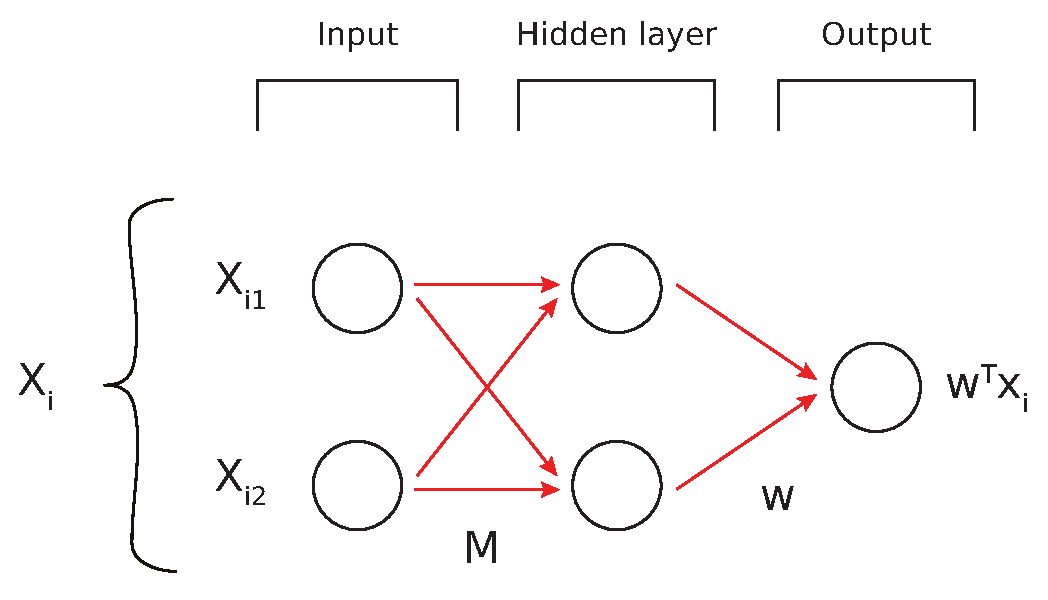
\includegraphics[width=0.5\textwidth]{images/nn-multi.eps}}
    \caption{A graphical representation of a Neural Network with an hidden layer.}
    \label{fig:nn-multi}
\end{figure}

\subsection{Chain rule}
The chain rule states that given $\hat{y} = f(g(x))$ its derivative is:
$$ \frac{d\hat{y}}{dx} = \frac{f(g)}{dg} \cdot \frac{g(x)}{dx} $$

That formula can be seen as a Neural Network with one node as input, one as output and one in the hidden layer.
Its graphical representation can be viewed in Figure \ref{fig:nn-chain}.

\begin{figure}[h]
    \centering
    \subfigure{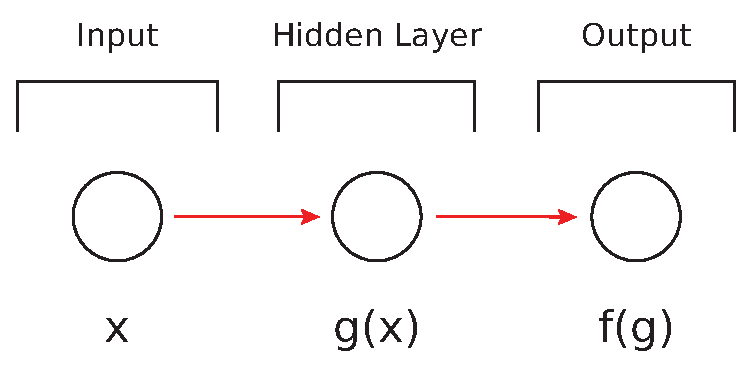
\includegraphics[width=0.5\textwidth]{images/nn-chain.eps}}
    \caption{A graphical representation of the chain rule.}
    \label{fig:nn-chain}
\end{figure}

\section{Backpropagation}
To better understand backpropagation, imagine having a fully connected Neural Network with:
\begin{itemize}
    \item $D$ nodes as input
    \item $J$ nodes in the hidden layer with $\tan$ as activation function
    \item 1 node as output with $\tan$ as activation function
\end{itemize}

This network has weights $M \in \mathbb{R}^{D \times J}$ between the first and the second layer,
and weights $w \in \mathbb{R}^{J} $ connecting the second layer to the third.

The minimization function is
$$\displaystyle \min_{M, w} \frac{1}{2} \sum_{i \in [1, N]} E(X, y)_i =
    \min_{M, w} \frac{1}{2} \sum_{i \in [1, N]} \{ \tanh[w^T \tanh(X_i M)] - y_i\}^2 $$

The final goal is to obtain:
\begin{multicols}{2}
    \begin{itemize}
        \item $\displaystyle \frac{dE_i}{dw}$
        \item $\displaystyle \frac{dE_i}{dM_{dj}}$
    \end{itemize}
\end{multicols}

In order to make the notation as light as possible, the function $\tanh(\cdot)$ is intended to be applied element-wise.
Moreover, the intermediate result $\tanh(M X_i)$ is denoted as $h_i$.

To compute the partial derivatives, we can start from the output layer and then use the intermediate calculations to compute
the partial derivatives of the previous layers.
In particular:
$$ \frac{dE_i}{dy_i} = \frac{1}{2} \cdot 2 \{ \tanh[w^T \tanh(M X_i)] - y_i\} = \tanh(w^T h_i) - y_i $$
$$ \frac{dE_i}{dw} = \frac{dE_i}{dy_i} \frac{dy_i}{dw} = \frac{dE_i}{dy_i} \{1 - \tanh^2[w^T \tanh(M X_i)]\} \tanh(X_i M) $$
$$ \frac{dE_i}{dh_i} = \frac{dE_i}{dy_i} \frac{dy_i}{dh_i} = \frac{dE_i}{dy_i} \{1 - \tanh^2[w^T \tanh(M X_i)]\} w $$

$$ \frac{dE_i}{dM_{dj}} = [\frac{dE_i}{dh_i} \circ \{\mathbb{1} - \tanh^2(X_i M)]\}_j X_{id}$$

The power of this technique is that it is possible to re-use values calculated for a particular partial derivative to lower the computational cost of computing the others.

The reasoning can be extended for multiple nodes as output.